\documentclass[12pt]{article}
\usepackage[margin=1in]{geometry} 
\usepackage{amsmath,amsthm,amssymb,amsfonts}
\usepackage{graphicx}
 
\newcommand{\N}{\mathbb{N}}
\newcommand{\Z}{\mathbb{Z}}
 
\newenvironment{problem}[2][Problem]{\begin{trivlist}
\item[\hskip \labelsep {\bfseries #1}\hskip \labelsep {\bfseries #2.}]}{\end{trivlist}}
%If you want to title your bold things something different just make another thing exactly like this but replace "problem" with the name of the thing you want, like theorem or lemma or whatever

\newenvironment{answer}[2][Answer]{\begin{trivlist}
\item[\hskip \labelsep {\bfseries #1}\hskip \labelsep {\bfseries #2.}]}{\end{trivlist}}

\begin{document}
 
%\renewcommand{\qedsymbol}{\filledbox}
%Good resources for looking up how to do stuff:
%Binary operators: http://www.access2science.com/latex/Binary.html
%General help: http://en.wikibooks.org/wiki/LaTeX/Mathematics
%Or just google stuff
 
\title{AST 231: Problem Set 1}
\author{Your Name Goes Here}
\maketitle
 
\begin{problem}{1}
The Solar Constant is about 1365 W/m$^2$. Calculate the distance from a 100 W light bulb at which its flux has the same value as the Solar Constant. Verify your result by holding your hand at that distance from the light bulb, but PLEASE do not BURN yourself due to an incorrect calculation!
\end{problem}

\begin{answer}{1}
Your answer goes here. Here's a sample formula to illustrate writing equations in Tex:
$$B_{\nu} = {2 h \nu^3 \over c^2}{1 \over e^{h \nu \over {k T}}-1}$$
\end{answer}

\begin{problem}{2}
A star that appeared to be single was measured to have V = 12.13 and B-V = 1.28. On closer inspection with HST it was found that this star is actually a visual binary, with component B being 0.90 mag fainter in V and 1.80 mag fainter in B than component A. Calculate the V magnitude and B-V color of each component.
\end{problem}

\begin{answer}{2}
Your answer goes here. 
\end{answer}

\begin{problem}{3}
Photometric data on a star are given in the table below. For your convenience, I also provide the flux density of a zero magnitude star and effective wavelengths of the filters for the photometric system in which the star was observed. The flux densities are in Jansky's (Jy), a favorite unit of infrared and radio astronomers. Be careful, because the Jy is a unit of F$_\nu$, not F$_\lambda$. There is a link on the course Moodle page to a Web site that will help you do the conversions correctly. Plot the tabulated data on a $F_\lambda$ versus log ($\lambda$) diagram. Make the scale be W/m$^2$/micron, as on the example, with wavelength expressed in microns. On the same diagram plot the blackbody curve (Planck function) with the temperature that you think best fits the data. In other words, you are using the spectral energy distribution (fondly called the SED by most astronomers) to estimate the effective temperature of the star. Be sure to state the effective temperature that you derive for the star by this method. 
\bigskip
\smallskip

\begin{tabular} {cccccc}

Filter & V & I & J & H & K \\
\hline
\hline
Magnitude & 16.11 & 14.47 & 13.42 & 12.74 & 12.47 \\
Effective Wavelength (in microns) & 0.545 & 0.798 & 1.25 & 1.65 & 2.20 \\
Zero mag Flux Density (Jy) & 3636.0 & 2416.0 & 1670.0 & 980.0 & 620.0 \\
\hline

\end{tabular}

\end{problem}


\begin{answer}{3}
Your answer goes here. As an example, here is how you include a pdf file of your plot, I have included one here. The file SamplePDF.pdf must be in the same directory as your tex file or must have the proper path to it.

\end{answer}

\bigskip
\bigskip

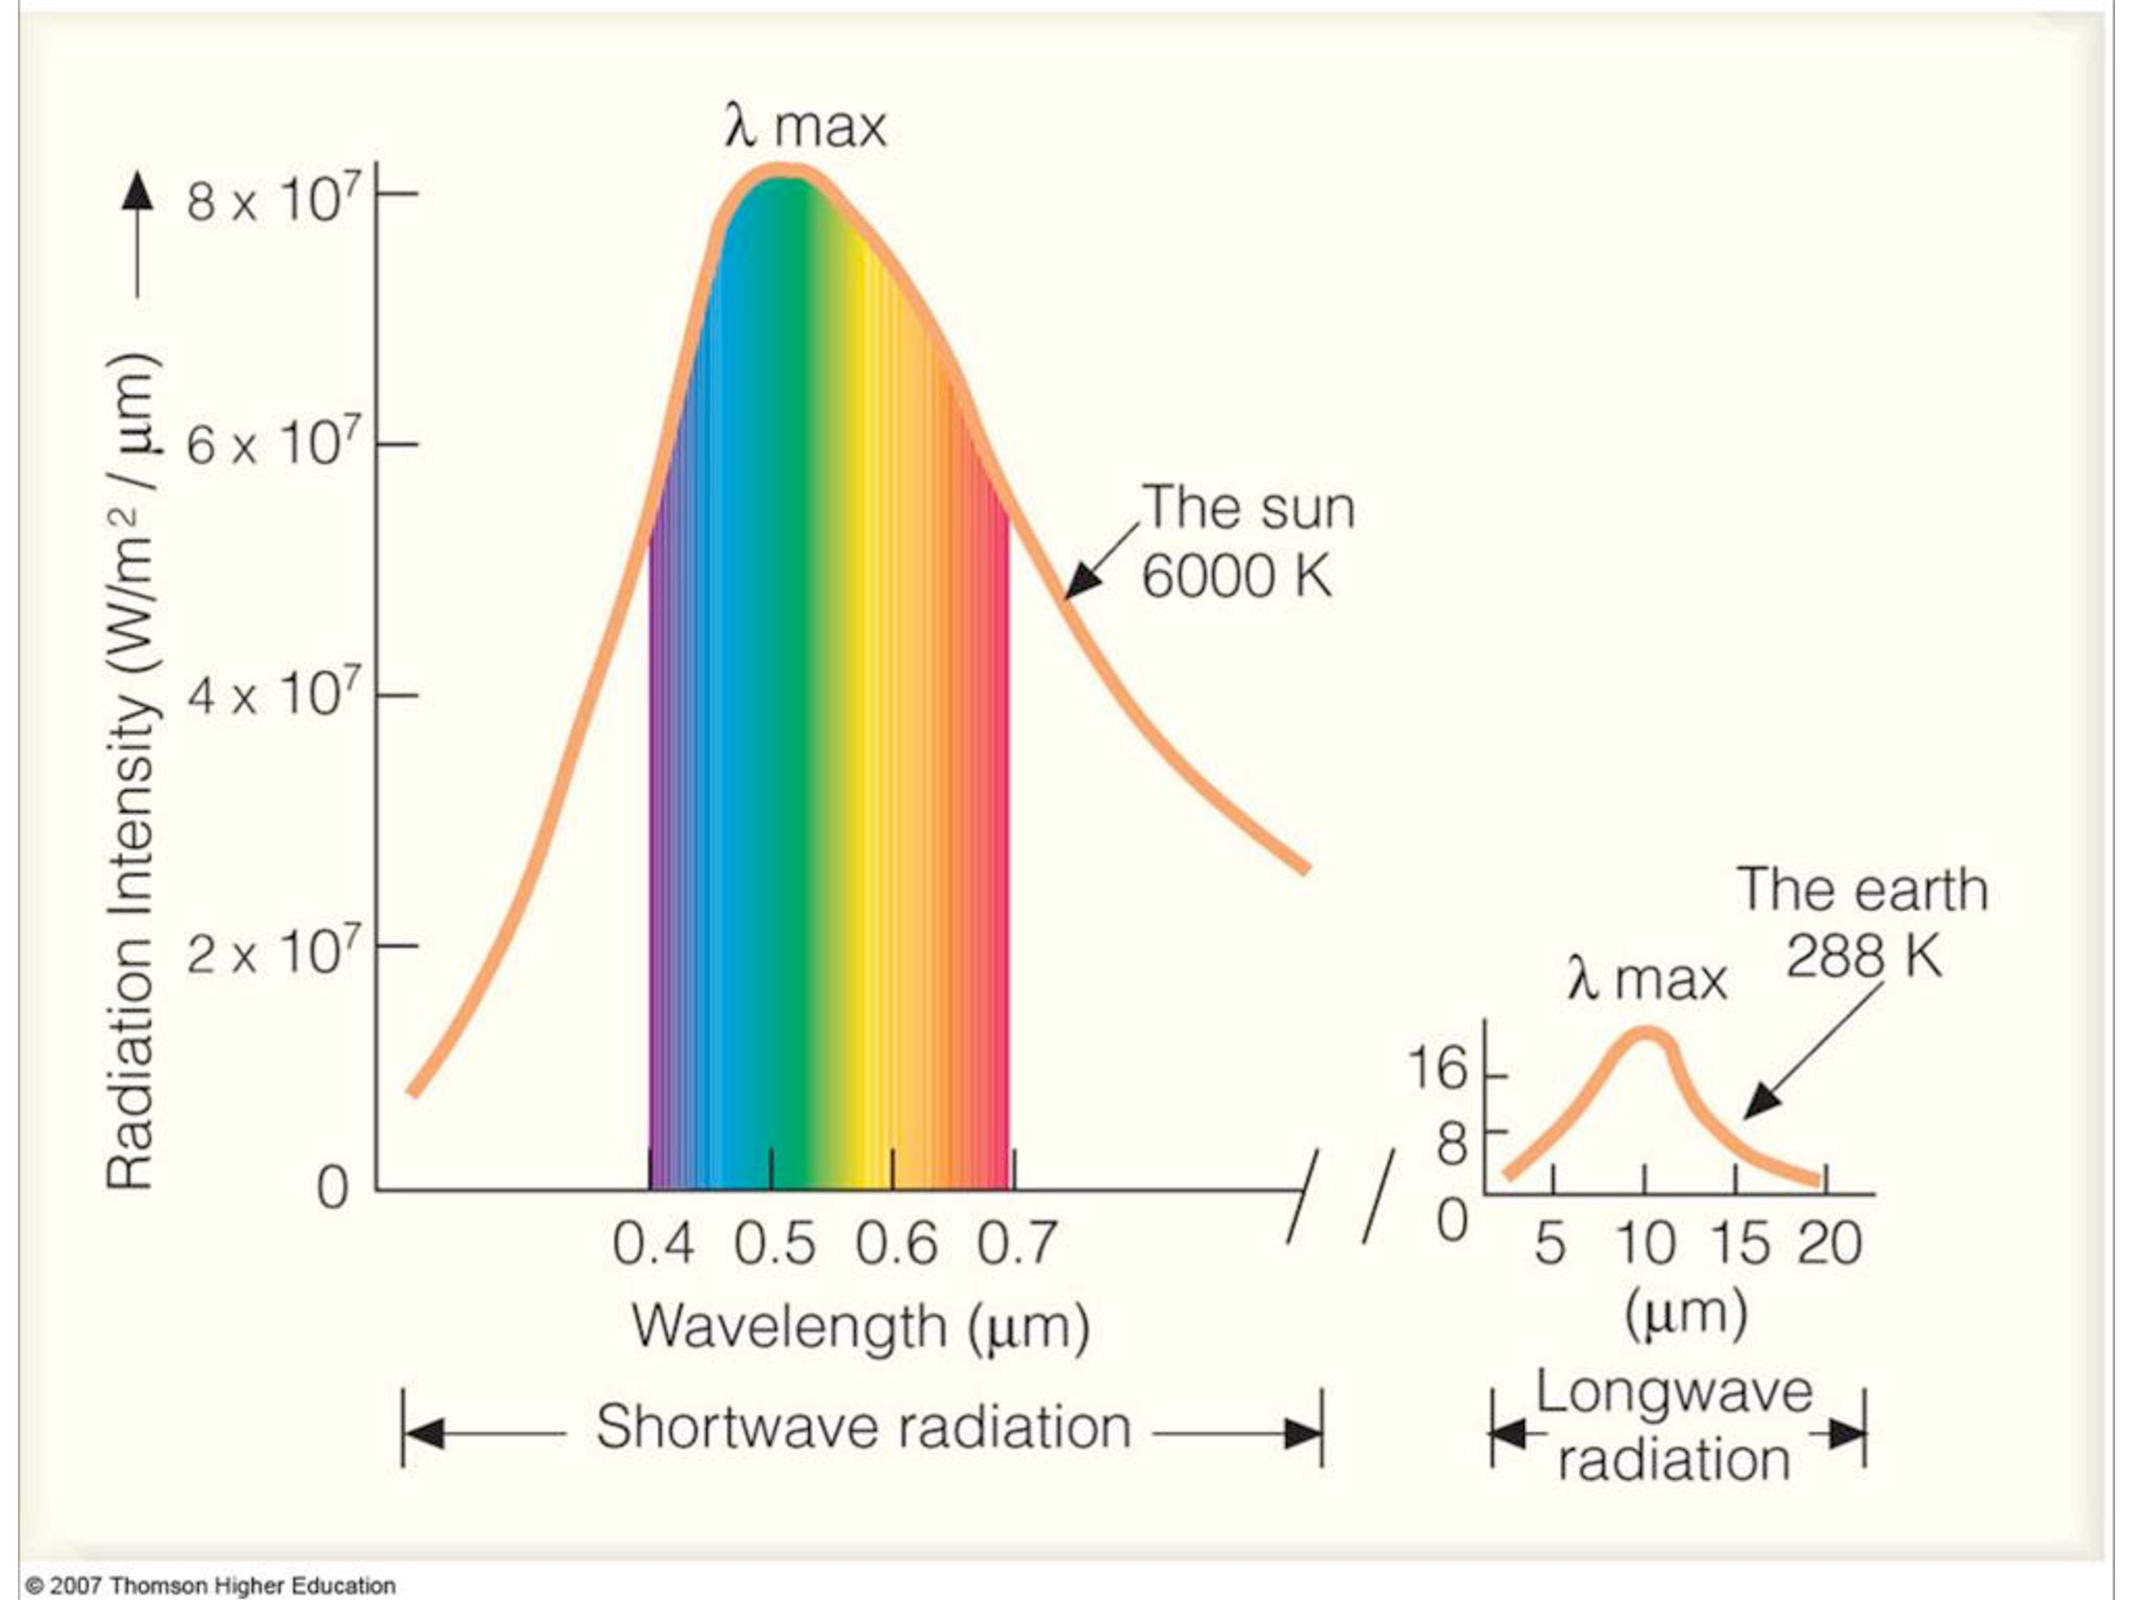
\includegraphics [scale=0.4] {SamplePDF}
 
\end{document}